\renewcommand\thesection{\arabic{section}}
\renewcommand\thesubsection{\thesection.\arabic{subsection}}


\textbf{Goal}:

Ideally, this step focuses on estimating the dimensions of the wood knots, using the built-in iPhone Measure API and/or a machine learning model to correctly calculate the exact size of the bounding box of the detected wood knots in reality. 


\begin{figure}[ht]
  \centering
   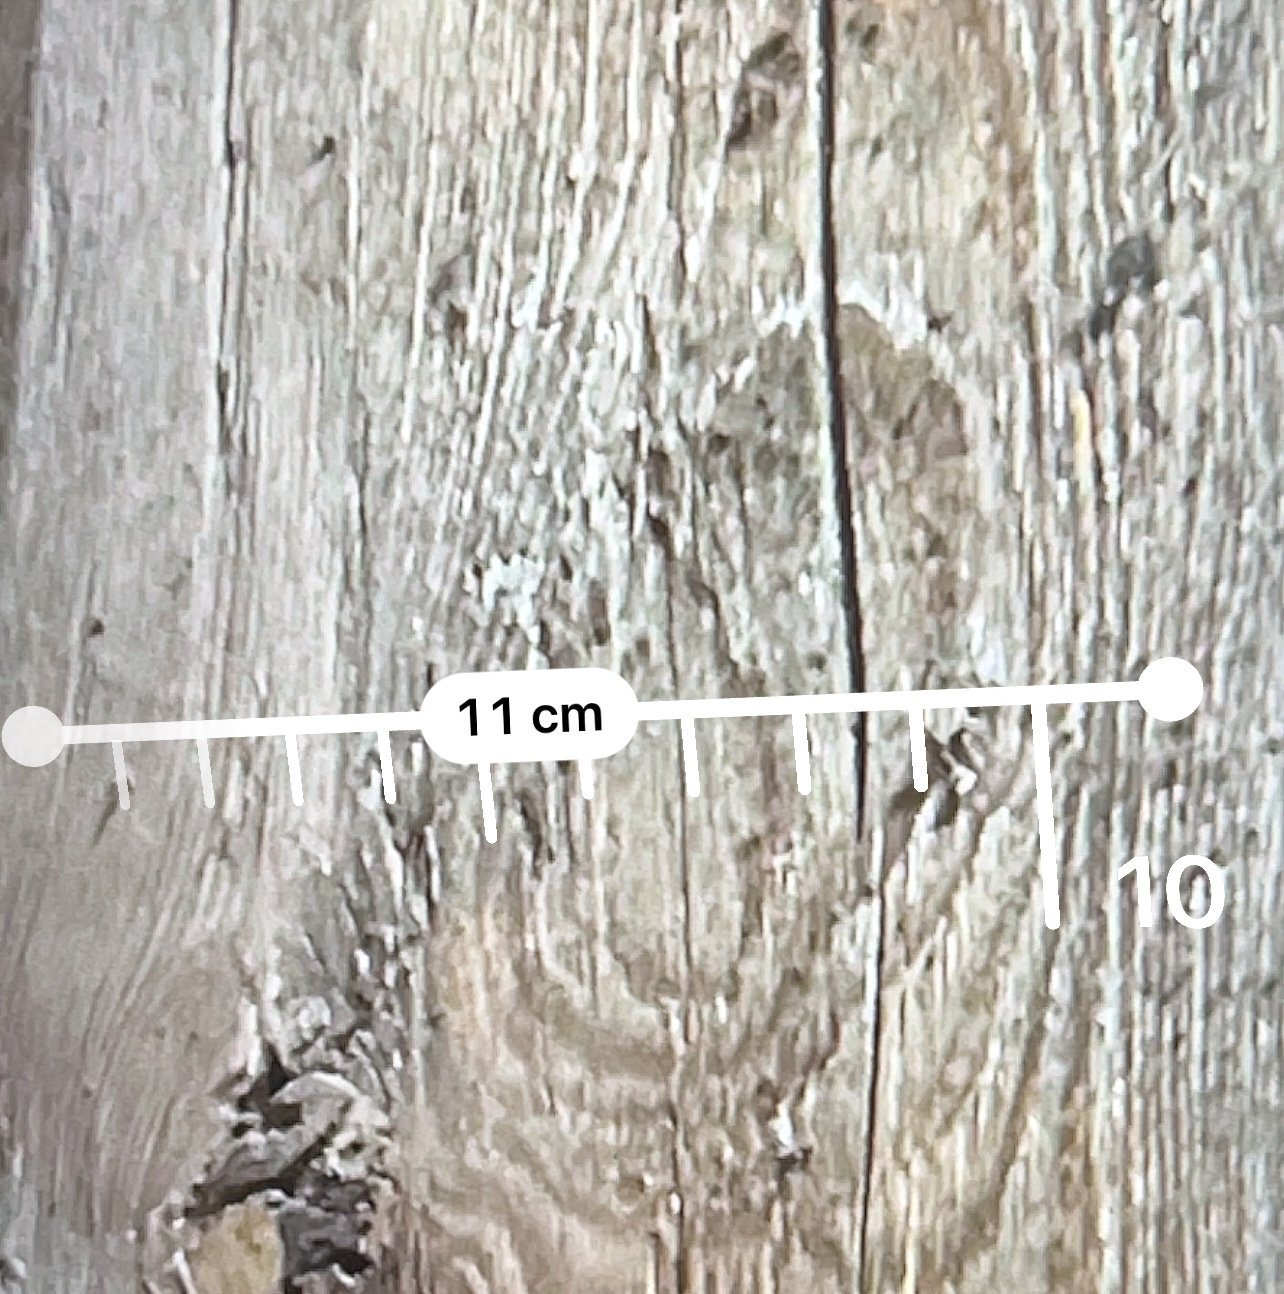
\includegraphics[width=.5\textwidth]{Master Thesis/Images/Section_3/3_iphone_measure.jpg}
  \caption{Mesurement using Measure App in iPhone}   
  \label{fig:iphone_mea}
\end{figure}  

\hspace*{\fill}

\textbf{Dataset}:

The dataset for measurement estimation required a concrete annotation for the pixel-dimensional bounding box in the image and its associated physical dimension. The creation of this specific dataset would only be considered after the insufficient measurement via the iPhone API.

\hspace*{\fill}

\textbf{Potential methods}:

Apple offers various APIs to access data from sensors such as Lidar or Gyroscope. It is also possible to access the measurement API~\footnote{https://developer.apple.com/documentation/foundation/measurement} in the iPhone supported by Apple's ARKit. (Figure~\ref{fig:iphone_mea}) Alternatively, it is also possible to build a machine learning model to estimate the dimension without a sensor. This method would require a large amount of annotated images with the size of the bounding box of wood knots both in pixels and in centimetres, which would be a much more time-consuming task and may also lead to greater bias than using the sensor. 


In conclusion, the first attempt would be to use the API in the iPhone to measure the actual dimension of a standard image and calculate the scale of the conversion from image to actual size. Then it is possible to use the standard image to calibrate the other images that are assumed to have been taken under similar circumstances and calculate the target measurement using the scale.

\hspace*{\fill}

\textbf{Output}:

The output will be one data group for each bounding box, which contains the dimension of the square bounding box and the distance from the border of the bounding box to wooden beam boundary.

\begin{figure}[ht]
    \begin{subfigure}[b]{0.3\textwidth}
        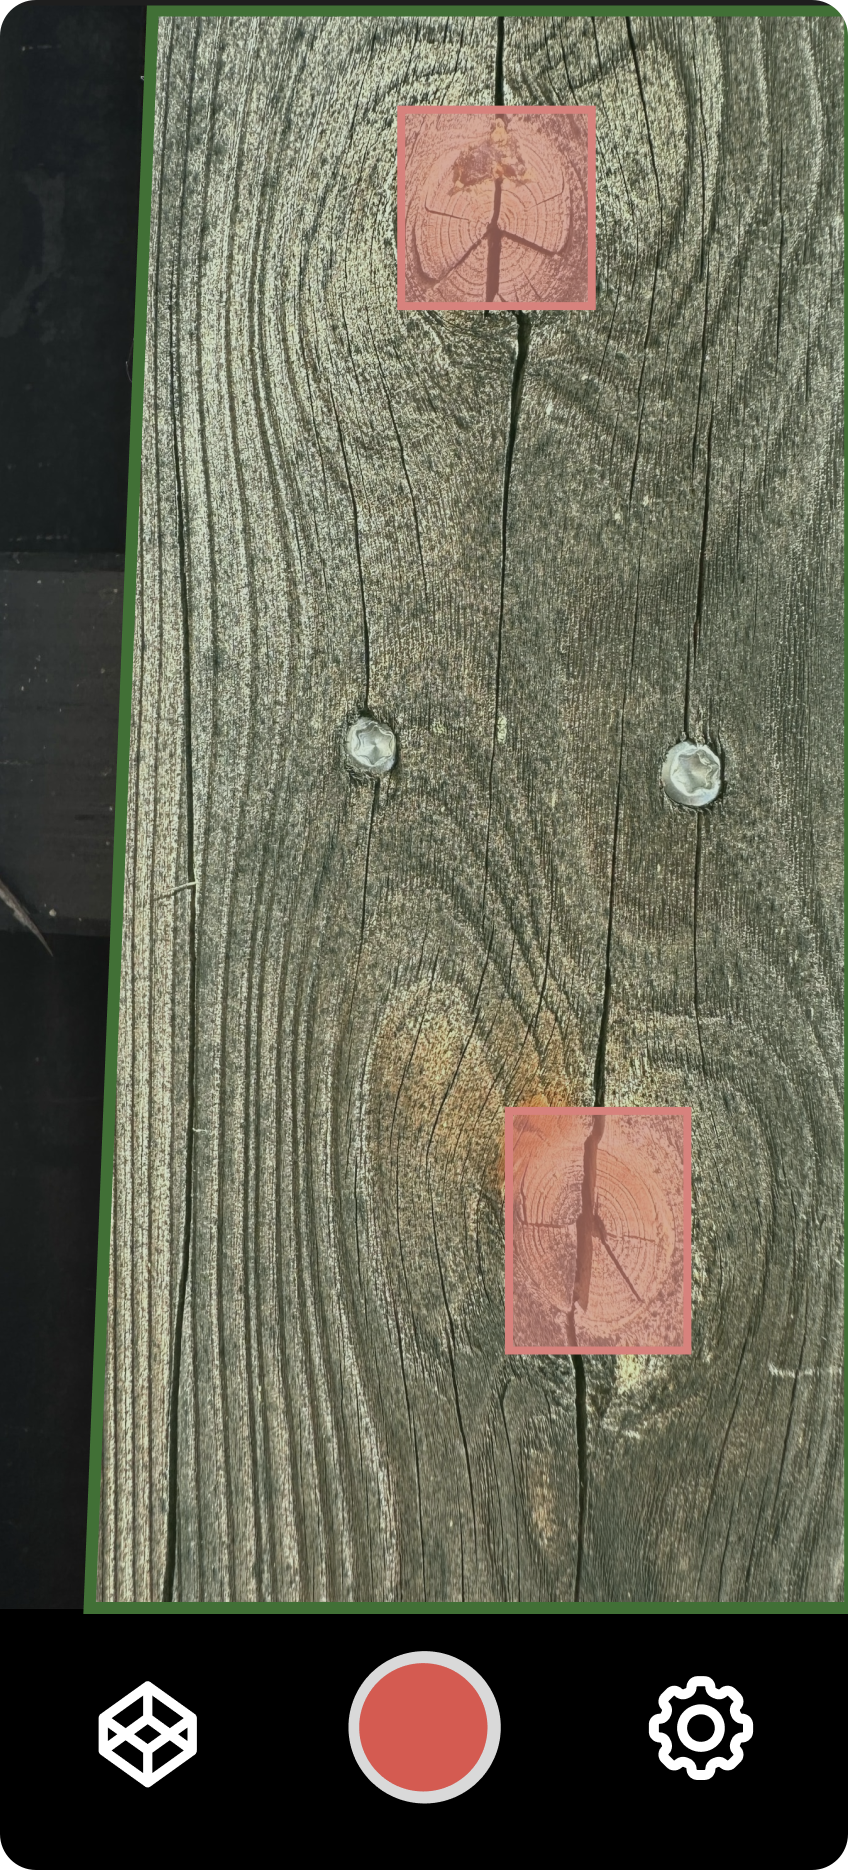
\includegraphics[width=0.7\textwidth]{Master Thesis/Images/Section_3/Mock/3-Mock3.png}
    \end{subfigure}
     \hfill
    \begin{subfigure}[b]{0.3\textwidth}
        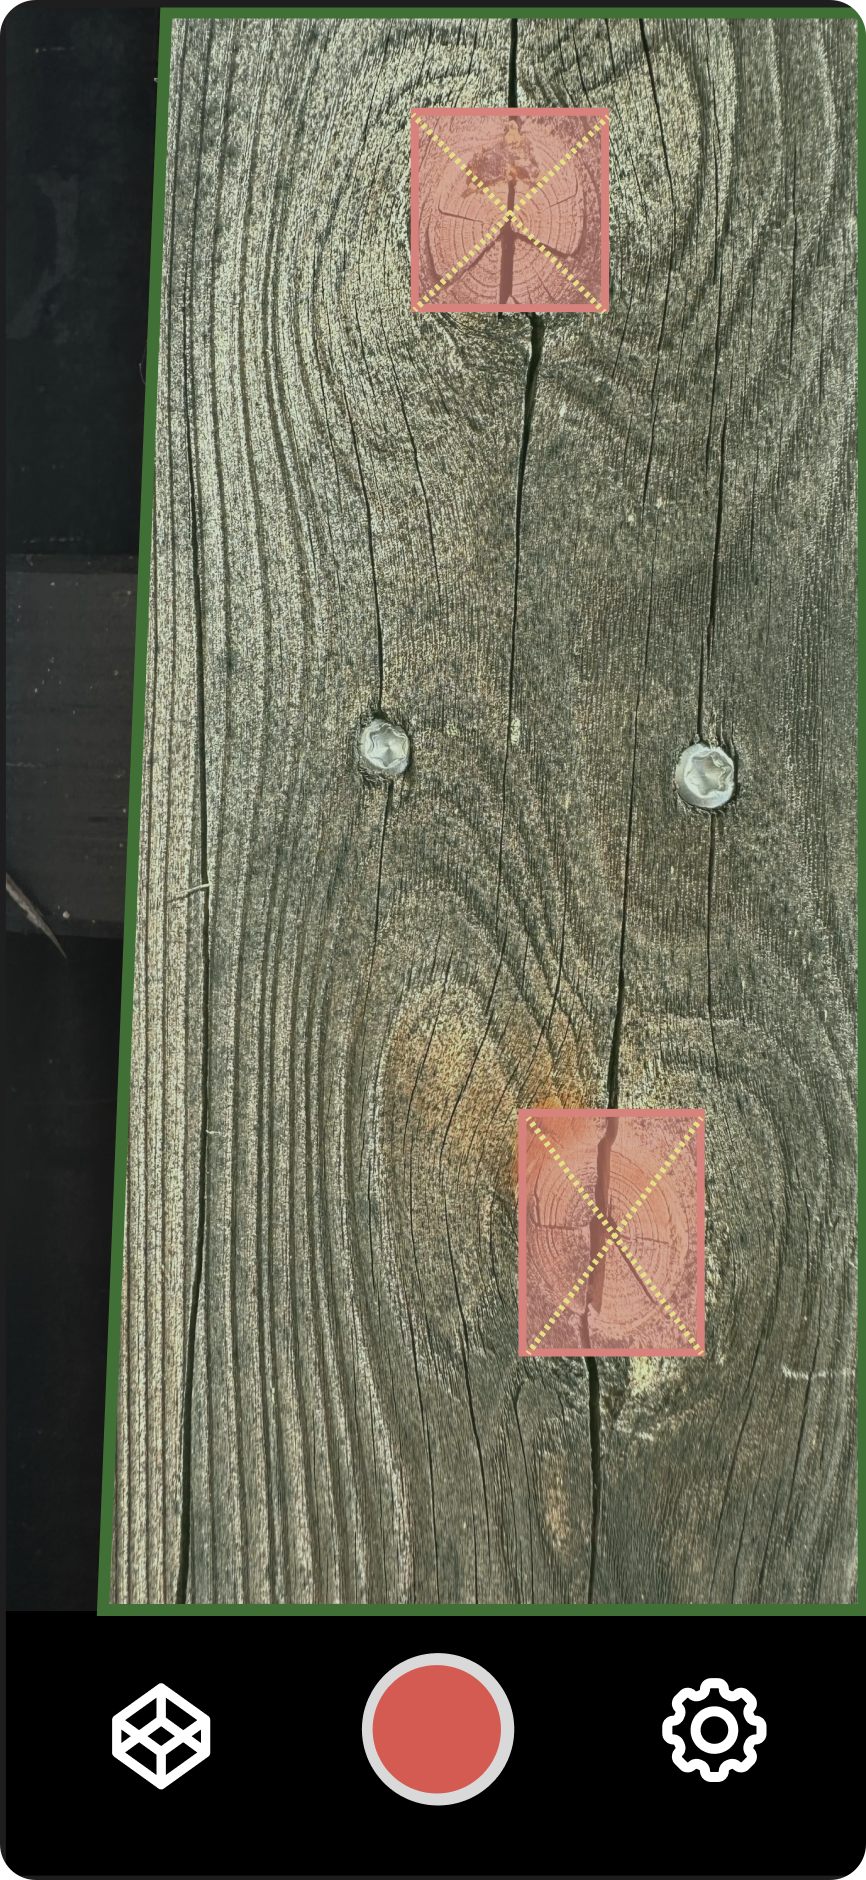
\includegraphics[width=0.7\textwidth]{Master Thesis/Images/Section_3/Mock/3-Mock4.png}
    \end{subfigure}
     \hfill
    \begin{subfigure}[b]{0.3\textwidth}
        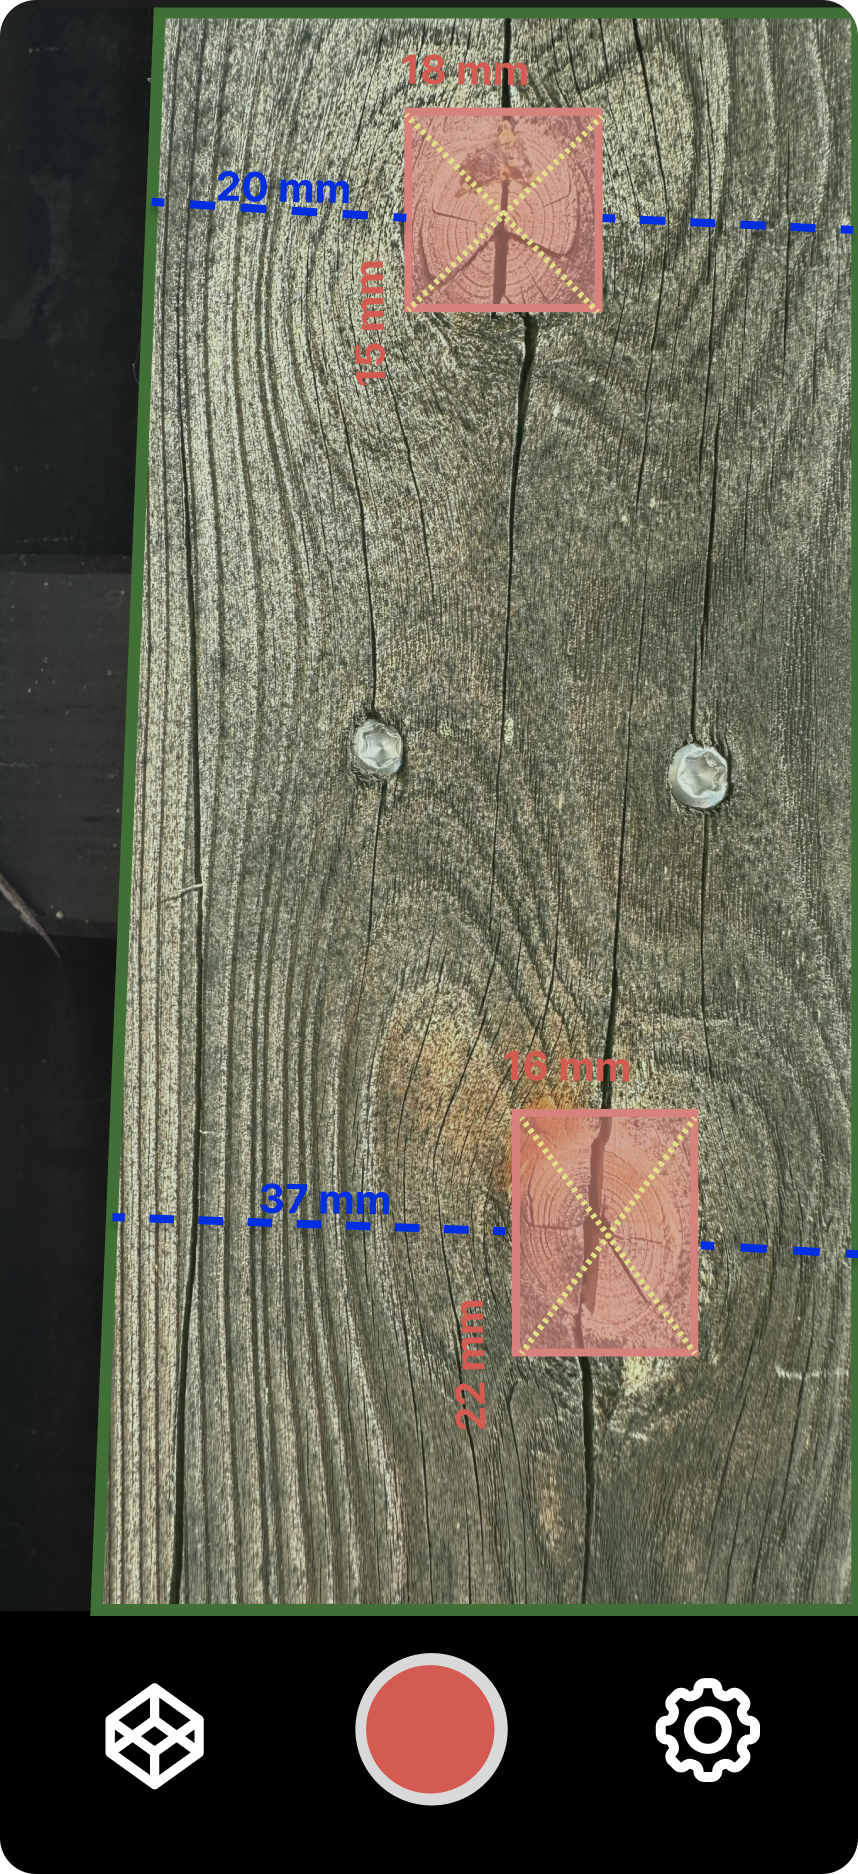
\includegraphics[width=0.7\textwidth]{Master Thesis/Images/Section_3/Mock/3-Mock5.png}
    \end{subfigure}
  \caption{Mocked-up output after dimension estimation of wood knots and distance to the boundary of wooden beams.}   
    \label{fig:mock3}
\end{figure}  
